\documentclass[11pt, a4paper]{article}
\usepackage[T1]{fontenc}
\usepackage{courier}

\usepackage[english, russian]{babel}

\usepackage{graphicx, geometry}
\usepackage{multicol}

\usepackage{amsmath}
\usepackage{cases}

\usepackage{fancyhdr}
\pagestyle{fancy}
\fancyhf{}
\fancyhead[C]{\thepage}

\graphicspath{ {./images/} }

\setcounter{page}{4}
\newgeometry{top=2cm, bottom=2cm, left=2.2cm, right=2.2cm}
\setlength{\columnsep}{0.8cm}

\setlength{\headwidth}{17.1cm} 

\begin{document}
\vspace*{-3em}  \centerline{\texttt{АНДРЕЙ НИКОЛАЕВИЧ КОЛМОГРОВ}}
\vspace*{0.8em}
\begin{multicols*}{2}
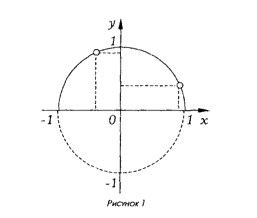
\includegraphics{picture1}
дем считать знаком извлечения арифмeтического квадратного корня. Равенство 
\begin{equation*}
     \hspace*{2.75cm} y = \sqrt{1 - x} \hspace*{2.75cm} \mbox{\raggedright{(1)}}
\end{equation*}
обозначает, что выпонены условия
\begin{equation*}
     \hspace*{1.4cm} x^2 \leq 1, \:\: y \geq 0, \:\: x^2 + y^2 = 1. \hspace*{1.4cm} \mbox{\raggedright{(2)}}
\end{equation*}
\hspace*{0.35cm} Точки, координаты которых удовлетворяют этим условиям, образуют полуокружность, изображенную на рисунке 1.\\
\hspace*{0.4cm} Рисунок 1 делает наглядными следующие факты, которые вы можете доказать и чисто алгебраическим путем:\\
\hspace*{0.5cm} 1) формула \mbox{\raggedright{(1)}} позволяет для любого $x$, удовлетворяющего условиям
\begin{equation*}
     \hspace*{2.6cm} -1 \leq x \leq 1, \hspace*{2.8cm} \mbox{\raggedright{(3)}}
\end{equation*}
вычислить соответствующее ему $y$, которое удовлетворяет неравенствам
\begin{equation*}
     \hspace*{2.85cm} 0 \leq y \leq 1; \hspace*{2.85cm} \mbox{\raggedright{(4)}}
\end{equation*}
\hspace*{0.55cm} 2) каждому $y$, удовлетворяющему неравенствам \mbox{\raggedright{(4)}}, соответствует хоты бы одно такое $x$, которому по формуле  \mbox{\raggedright{(1)}} соответствует это заданное $y$.\\
\hspace*{0.5cm} Можно сказать, что формула \mbox{\raggedright{(1)}} задает отображение множества чисел x, удовлетворяющих неравенствам \mbox{\raggedright{(3)}}, на множество чисел, подчиненных неравенствам \mbox{\raggedright{(4)}}.
Математики часто (особенно в последнее время) для обозначения отображений употребляют стрелку. Занимающее нас отображение можно записать при помощи стрелки так:
\begin{equation*}
	 \hspace*{2.62cm} x  \to \sqrt{1 - x^2}  \hspace*{2.62cm} \mbox{\raggedright{(5)}}
\end{equation*}
\hspace*{0.6cm} Заметьте: \textit{отображение полностью определено, если а) задано множество $E$, которое отображается; б) для каждого элемен- 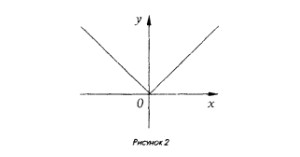
\includegraphics{picture2} та $x$ этого множества $E$ задан элемент $y$, на который элемент $x$ отображается.} \\
\hspace*{0.4cm} Множество всех значений $y$ обозначим буквой $M$. В первом примере $E$ - множество чисел, удовлетворяющих условию \mbox{\raggedright{(3)}}, а $M$ -- множество чисел, удовлетворяющих условию \mbox{\raggedright{(4)}}. \\
\hspace*{0.4cm} \textbf{Пример 2.} Правила
\begin{equation*}
     1)\: x \to \sqrt{x^2}  \hspace*{4.8cm} 
\end{equation*}
\begin{equation*}
     2)\: x \to \begin{cases}
    x, \: \text{если} \: x \geq 0\\
   -x, \: \text{если} \: x < 0
\end{cases}  \hspace*{2.38cm} 
\end{equation*}
определяют одно и то же отображение
\begin{equation*}
     \hspace*{3.1cm} x \to |x| \hspace*{3.1cm} \mbox{\raggedright{(6)}}
\end{equation*}
действительных чисел $x$ на их модули (абсолютные велечины) (рис. 2). \\
\hspace*{0.3cm} Отображение \mbox{\raggedright{(6)}} отображает множество всех действительных чисел
\begin{equation*}
     R = (-\infty;+\infty)
\end{equation*}
на множество
\begin{equation*}
     R_+  = [0;+\infty)
\end{equation*}
неотрицательных действительных чисел.\\
\hspace*{0.4cm} Вместо слова \textit{отображение} можно говорить \textit{функция} и записать отображение \mbox{\raggedright{(5)}} так:
\begin{equation*}
	\hspace*{2.33cm} f(x)  = \sqrt{1 - x}, \hspace*{2.33cm} \mbox{\raggedright{(7)}}
\end{equation*}
а отображение \mbox{\raggedright{(6)}} так:
 \begin{equation*}
	\hspace*{2.75cm} f(x) = |x|. \hspace*{2.75cm} \mbox{\raggedright{(8)}}
\end{equation*}
\hspace*{0.25cm} Областью определениея функции \mbox{\raggedright{(8)}} является множество всех действительных чисел R. Множеством ее значений являеется множество R+ неотрицательных действительных чисел. \\
\hspace*{0.25cm} \textbf{Пример 3.}  Петя, Коля, Саша и Володя живут в комнате общежития. На февраль они установили такой график дежурств:
\end{multicols*}
\end{document}